\section{Introduction}
%\label{sec:introduction}

%The introduction contains: 
%\begin{itemize}
%	\item Setting up the context of automated driving
%	\item Giving some background information about the hazard analysis and risk assessment in the ISO~26262 standard
%	\item The gap (the problem) We currently have this as a separate chapter, we could move it to introduction depending on the length. 
%	\item our contribution. 
%	\item paper structure
%\end{itemize}

New developments in the automotive industry towards higher levels of automation are introducing new safety concerns for vehicles. Test procedures and performance measures need to be adapted for evaluation of vehicles with an Automated Driving (AD) system. The safety and reliability of the AD vehicles must be validated in principle for all possible traffic situations that an AD system may encounter on the road, before these systems can be taken into production.

Scenario-based safety validation for automated driving is one of the proposed approaches that is broadly supported by the automotive community. This is reflected in the ISO/PAS~21448:2019 standard on the safety of th intended functionality (SOTIF) \cite{ISO21448}. Related projects in Germany (Pegasus \cite{putz2017pegasus}), The Netherlands (StreetWise \cite{elrofai2018scenario}), and Singapore \cite{ploeg2018cetran} strongly support this approach. Risk assessment is an essential component of the safety validation as it indicates the acceptance criteria of the AD system.

The ISO~26262:2018 \cite{ISO26262} captures the state of the art in automotive functional safety. It defines the safety lifecycle and the related safety activities such as Hazard Analysis and Risk Assessment. Other methodologies, such as STPA \cite{leveson2013stpa}, give guidelines on safety engineering based on systems theory. From the mentioned sources, the only one that offers a framework for measuring risk is ISO~26262. It defines risk as:
\begin{definition}[Risk \cite{ISO26262}]
	The combination of the probability of occurrence of harm and the severity of that harm.
\end{definition}

ISO~26262:2018 gives guidelines to assess risk based on vehicle level hazardous events. A hazardous event is the combination of a vehicle level hazard with operational situation or scenario. It requires analyzing each hazardous event risk individually based on three parameters of Severity, Probability of exposure, and Comparability. The combination of these parameters contributes to constructing the Automotive Safety Integrity Level (ASIL). In this framework, each parameter is quantified in three or four levels that construct the ASIL ranking A, B, C, D, and QM, where ASIL A represents the least critical level and in ascending order, ASIL D the most critical level. Quality Management (QM) means that the identified hazard is not critical enough for the safety processes, and the quality management system of the manufacturer should suffice for reducing the risk. We depict the ASIL ranking graph in \cref{Fig:ASILGraph}. 

\begin{figure}[b]
	\centering
	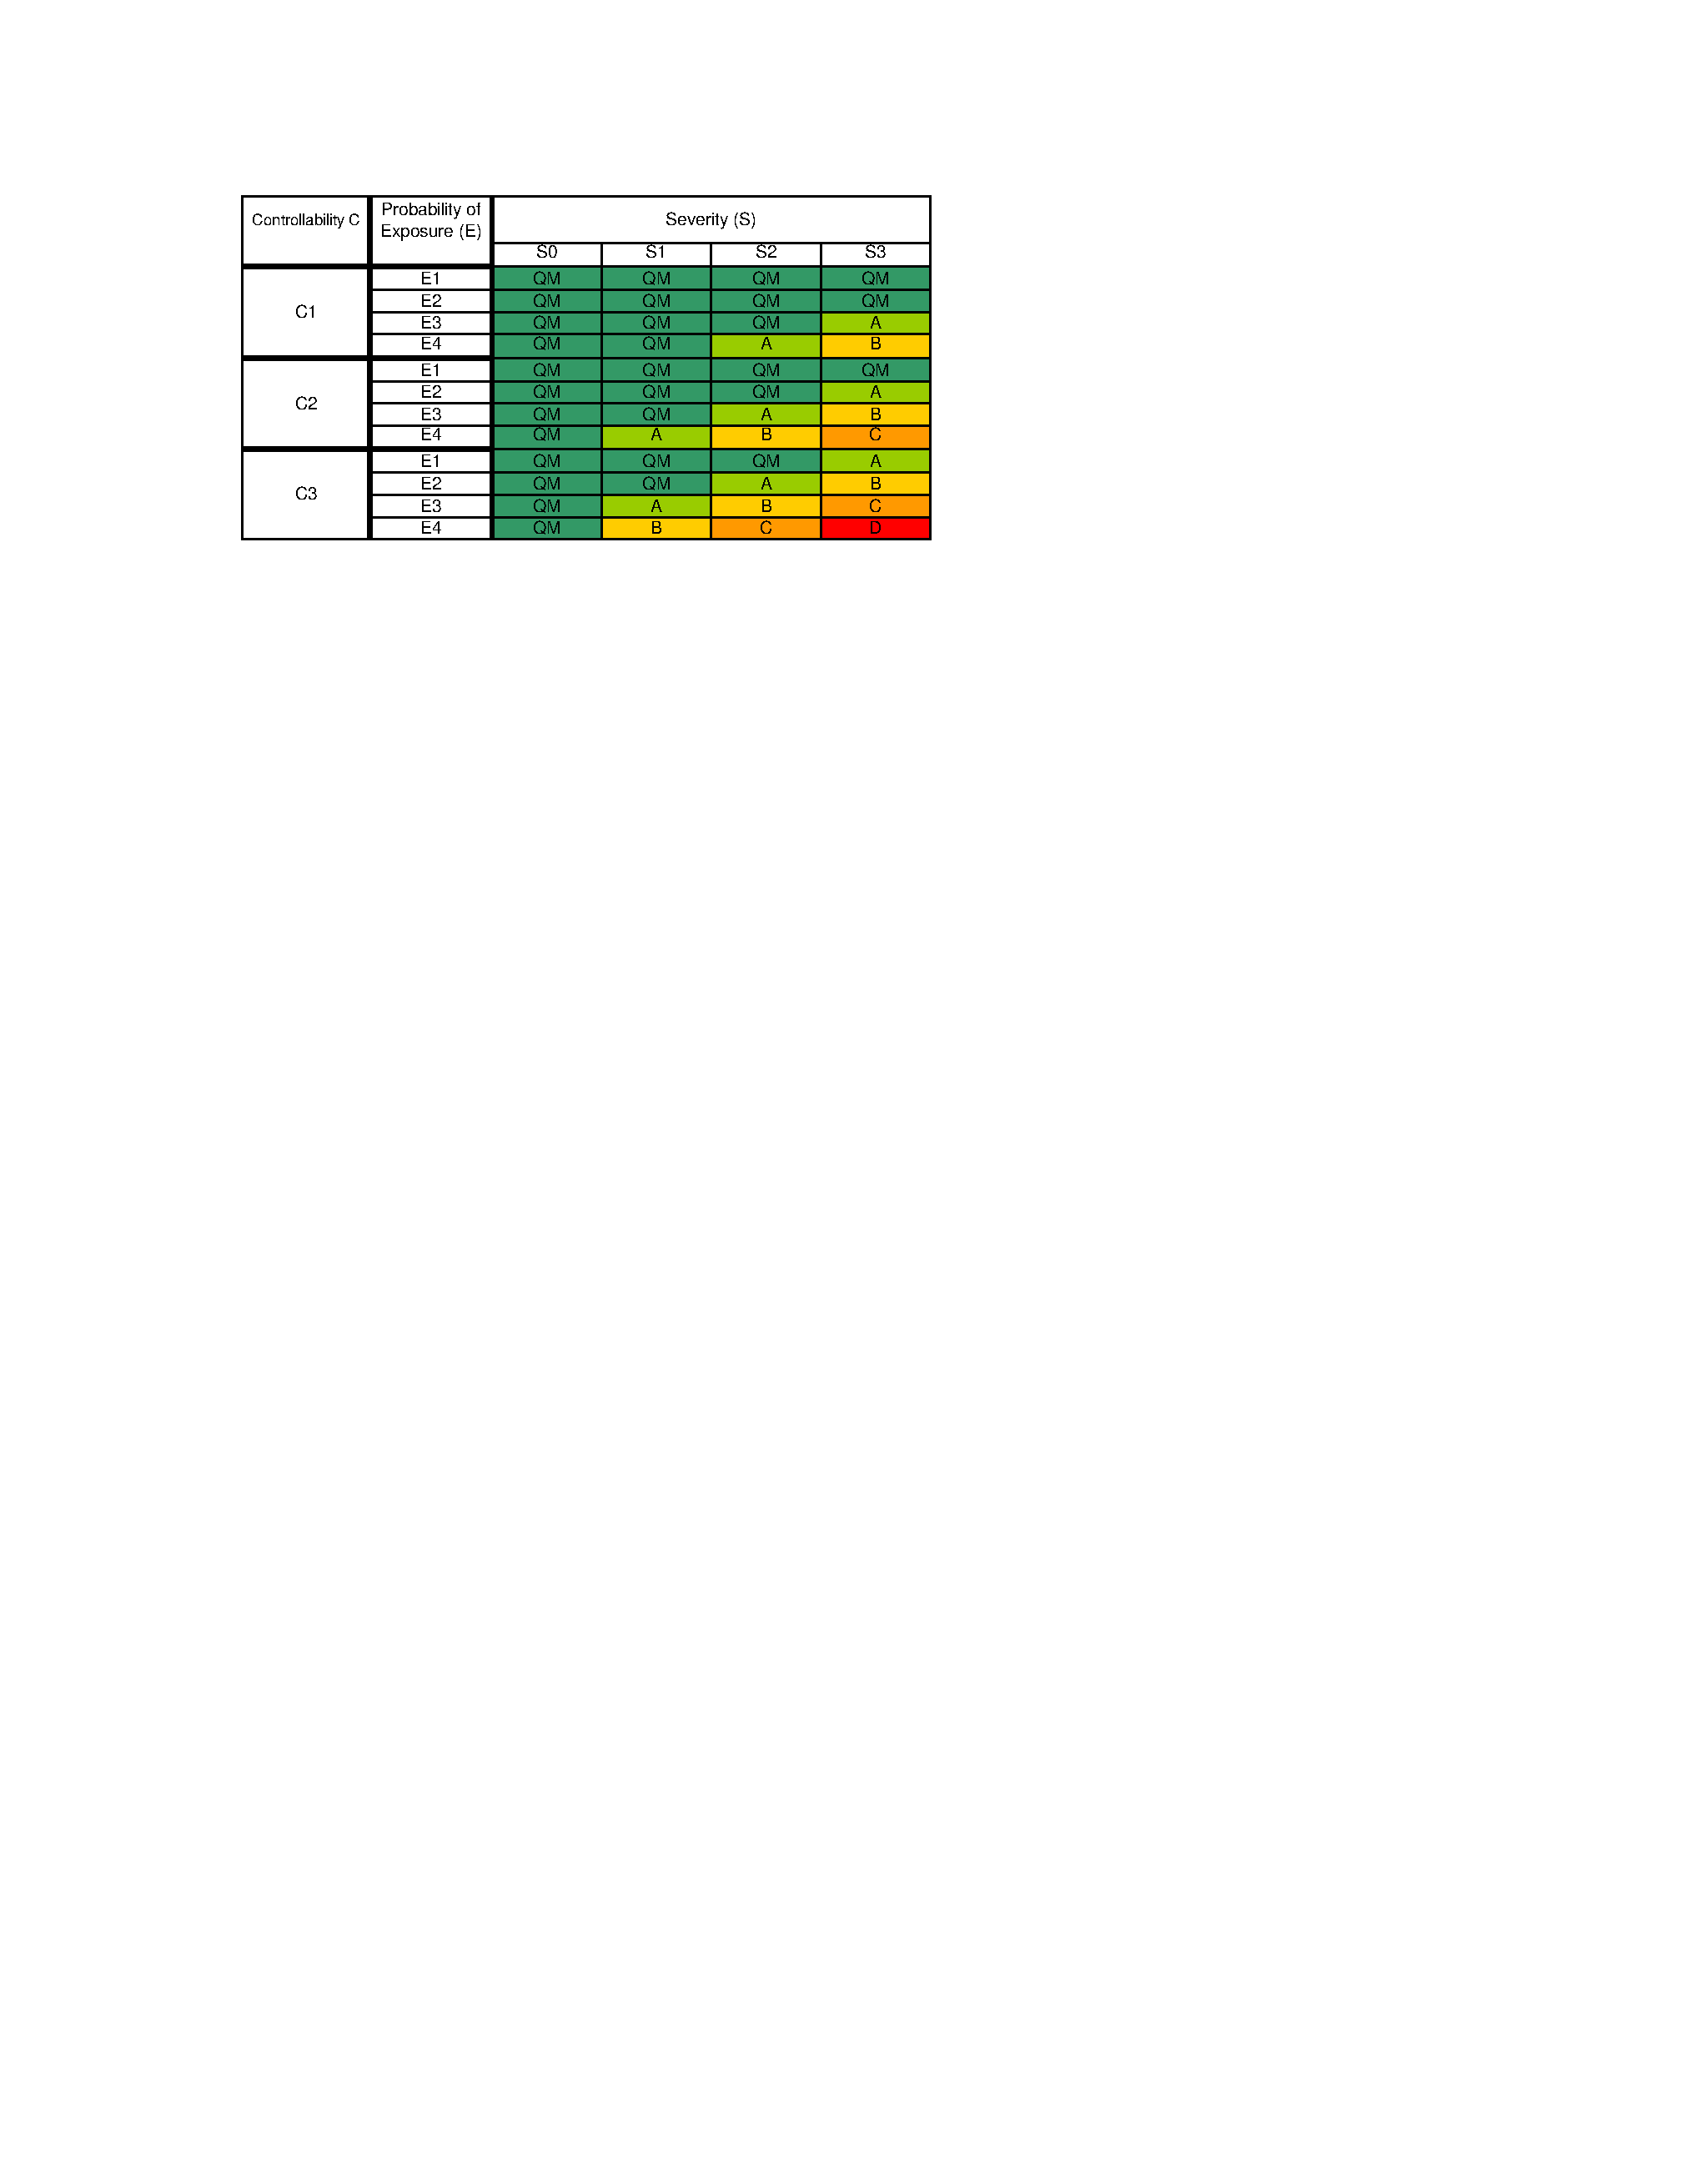
\includegraphics[width=0.6\linewidth]{./figures/ASIL}
	\caption{ASIL risk assessment graph.}
	\label{Fig:ASILGraph}
\end{figure}

The ASIL methodology for risk assessment relies on the experts’ judgments of the three risk parameters. The ISO~26262:2018 provides some general guidelines for assessing these parameters. However, the assessment is for the most part subjective and dependent on the experts who carry it out. Moreover, it is only capable of evaluating the risk of a single (hazardous) event within the context of a generic operational situation.

The alternative methodology proposed in STPA has the means for providing a quantitative risk assessment as it provides the means for connecting the hazard identification to a control system and its characteristics. However, this method skips the risk assessment entirely and does not offer any solutions. 

We argue that as the automotive systems move towards higher automation levels, we require more formal methods for risk assessment. By quantifying risk assessment, we reduce the risk of subjective errors in the judgment. Risk quantification is a step towards run-time risk assessment for the autonomous systems.  

The objective of this paper is to introduce a method for assessment and quantification of the risk of a driving scenario taking into account the entire operational situations and their relations. This is achieved by calculating the probability of exposure to a certain scenario through analysis of real-world driving data. Next, we employ simulations to estimate the severity of the potential hazardous consequence of a scenario.


%likelihoods of the activities, and environmental conditions that constitute the cut-in scenarios. Monte Carlo simulations are employed for determining the outcome of the cut-in scenarios, e.g., a collision or a near miss, given a state-of-the-art highway pilot system
%The main limitation of the presented case study is the limited amount of data used. Furthermore, we applied the proposed method for only one type of driving scenario, while the full potential can be better demonstrated by applying the method to a wider range of scenarios.

The paper is structured as follows. We first present the proposed method for estimating the risk quantitatively. Next, we perform a case study to illustrate the method using real-world data. We end the paper with a discussion and a conclusion.
